\documentclass[titlepage]{article}
\usepackage{graphicx}
\usepackage{hyperref}
\usepackage{fancyhdr}

\title{ \textbf{final homework of computer workshop} \newline Iran University of science and technology \newline \newline shomare daneshjoii: 402522031}
\author{Parham Mohammadi }
\date{1402/11/06}


\begin{document}
\maketitle

\pagestyle{fancy}
\fancyhead[L]{1}
\fancyhead[R]{}

\tableofcontents
\newpage
\fancyhead[L]{1}
\fancyhead[R]{}
\section{Git and Github}
\subsection{ Repository Initialization and Commits}
first of all in github we build a repository in our github account. Then we build a workflow that contanis main.yml. This workflow compiles the latex file that we put in our repository. This workflow compile it tag by tag, so we have to push every commits by tags and latex file must be pushed section by section.This latex file must include sections for each category of the questions.
\subsection{ GitHub Actions for LaTeX Compilation}
At the beggining I thought I have to make a folder named .github and then make a folder named workflow in .github and then make main.yml file in workflow folder and then push it in repository, but i ran it and it didnt work, so I delete it and in Actios in repository I made a workflow that contains main.yml and I copied main.yml in held repository into my workflow and then it worked.
\section{ Exploration Tasks}
\subsection{Vim Advanced Features}
In this section we describe some vim advanced features :
\begin{enumerate}
\item Crtl + P : when we are in insert mode, we use vim and write a text , for example you write "printf" , if you want to write it again, you can write p and use Crtl + p and then it shows some words that starts with p and you can chose which of them you want to use.
\item gUw : in normal mode if you want to switch the word to the right of the cursor to upper case, you use this feature. you type gU2w to upper case two words.
\item Crtl + A or Crtl + X : in normal mode, when you want to change a number, to increment the number or to decrement the number use can use them, to to increment the number you use Crtl + A and to decrement the you use Crtl + X
\end{enumerate}
\subsection {Memory profiling}
\subsubsection {Memory Leak}
A memory leak is a program error that consists of repeatedly allocating memory, using it, and then neglecting to free it.
\newline in fact  a memory leak is a type of resource leak that occurs when a computer program incorrectly manages memory allocations. some ways that it might happen are below :
\newpage
\fancyhead[L]{2}
\fancyhead[R]{}
\begin{enumerate}
\item{when an object is stored in memory but cannot be accessed by the running code. }
\item{when a program fails to release memory that it has allocated dynamically.}
\end{enumerate}
\subsubsection {Memory profilers}
Valgrind is a programming tool for memory debugging, memory leak detection, and profiling.\newline Valgrind was originally designed to be a freely licensed memory debugging tool for Linux on x86, but has since evolved to become a generic framework for creating dynamic analysis tools such as checkers and profilers.\newline
In fact Valgrind is a virtual machine. Nothing from the original program ever gets run directly on the host processor. Instead, Valgrind first translates the program into a temporary, simpler form called intermediate representation (IR). After that a tool is free to do whatever transformations it would like on the IR, before Valgrind translates the IR back into machine code and lets the host processor run it. It also includes a GDB(The GNU Debugger (GDB) is a portable debugger that runs on many Unix-like systems and works for many programming languages) stub to allow debugging of the target program as it runs in Valgrind, with "monitor commands" that allow querying the Valgrind tool for various information.
\subsection{GNU/Linux Bash Scripting}
\subsubsection{fzf}
\begin{enumerate}
\item A fuzzy search is a technique that uses search algorithms to find strings that match patterns approximately. In fact a fuzzy search searches for text that matches a term closely instead of exactly. Fuzzy searches help you find relevant results even when the search terms are misspelled.
\item The command \texttt{"ls | fzf"}, combines the functionality of the "ls" command, which lists files and directories, with the interactive search interface provided by the "fzf" command. This combination is extremely useful when you want to navigate and find specific files or directories quickly within the terminal environment. By using \texttt{"ls | fzf"}, you can easily search through the list of files and directories, refining your search interactively until you locate the desired item. This command is a valuable tool for efficient file management and exploration in the command line.
\end{enumerate}
\newpage
\fancyhead[L]{3}
\fancyhead[R]{}
\subsubsection{Using fzf to find your favorite PDF}
\begin{enumerate}
\item Command to list the directory of all files with the extension .PDF: "fd -e pdf"
\item Command to use fzf to select a PDF from the data we gathered above: "fd -e pdf \texttt{| fzf"}
\end{enumerate}
\subsubsection{ Opening the file using Zathura}
Command to open the selected PDF file using Zathura: zathura  \$ (fd -e pdf \texttt{| fzf})" 
\section {Git and FOSS}
\subsubsection{README.md}
README.md added and filled completely
\subsection {Issue}
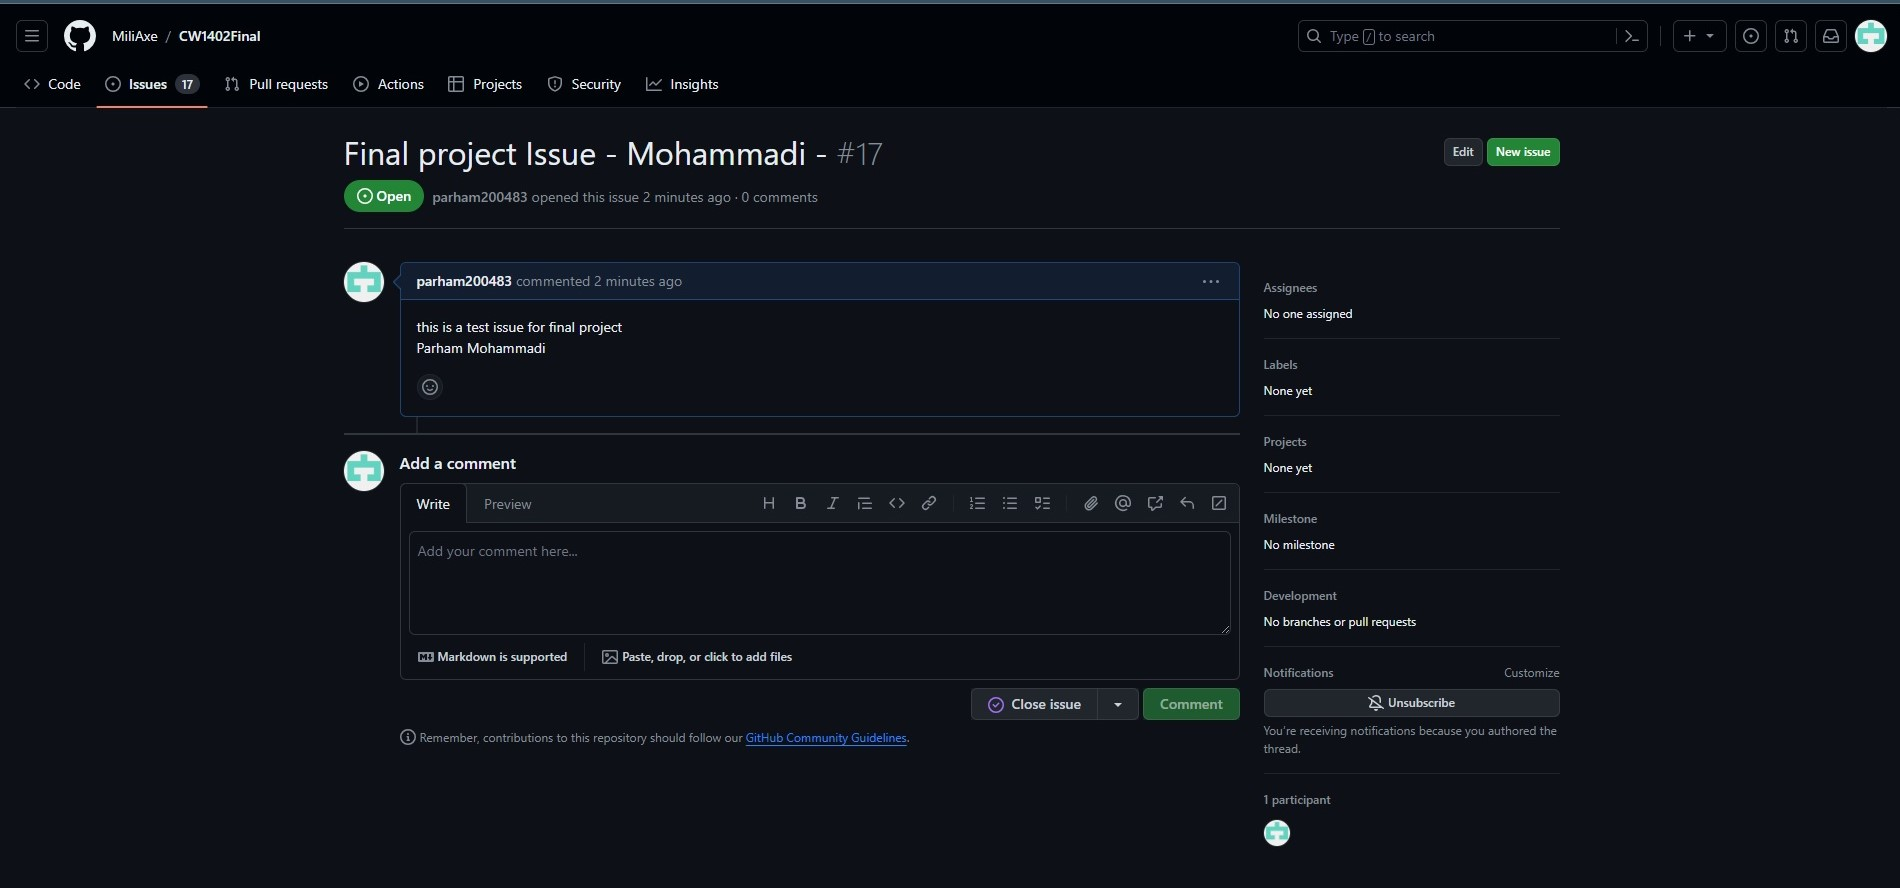
\includegraphics[width=\textwidth,height=\textheight,keepaspectratio]{final-project-Parham Mohammadi.jpg}
\newline \newline issue commited by parham200483 and named Final project Issue - Mohammadi -
\end{document}
